\chapter{Descripción del Proceso}
    \section{Proceso de gestión de Programas Académicos}
        \subsection{Jefe de Innovación Educativa de la Unidad Académica}
        \begin{figure}[!hbtp]
        	\centering
        	\hypertarget{BPMNG}{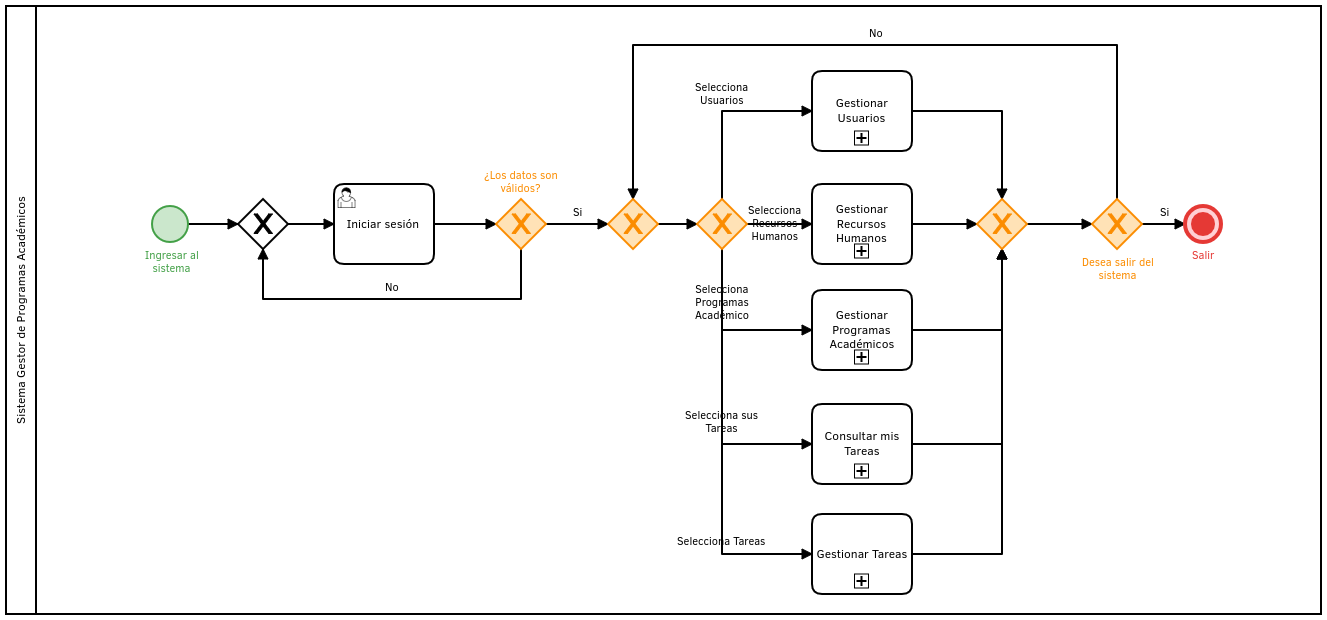
\includegraphics[width=\linewidth]{images/SP1/ProcesoGeneral}
        	\caption{Proceso General para el Usuario Jefe de Innovación Educativa}}
        	\label{BPMNG}
        \end{figure}
    
    	\subsubsection{Gestión de Recursos Humanos}
    	
        \begin{figure}[!hbtp]
        	\centering
        	\hypertarget{BPMNGRH}{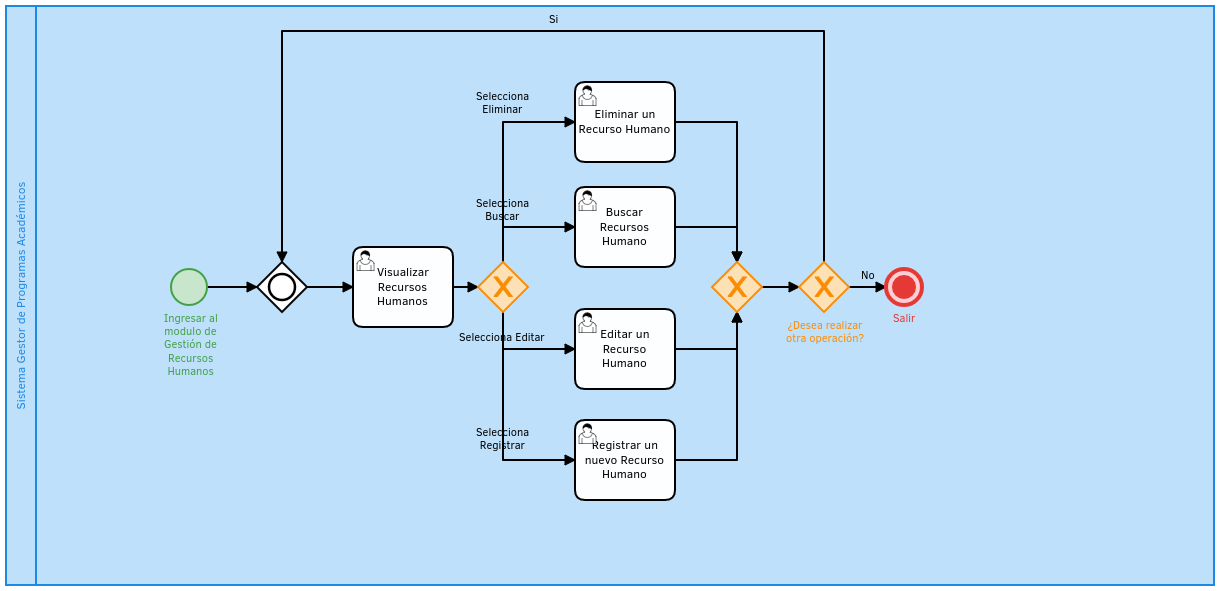
\includegraphics[width=\linewidth]{images/SP1/gestionRH.png}}
        	\caption{Subproceso de la gestión de Recursos Humanos}
        	\label{BPMNGRH}
        \end{figure}
        
        El Jefe de Innovación Educativa de la Unidad Académica accede al Sistema Gestor de Programas Académicos.\\
        
        Ingresa su matrícula y contraseña para iniciar sesión. En caso de errores de validación de sus datos, debe intentarlo de nuevo.\\
        
        Ya dentro del sistema, accede a la sección llamada ''Gestión de Recursos Humanos'' Aquí podrá consultar, visualizar, eliminar, modificar y agregar recursos humanos de la Unidad Académica bajo su cargo. \\
        
        Para agregar y/o editar un recurso humano, es necesario acceder a dos pantallas distintas. Es decir, no puede realizar ambas acciones de manera simultánea.\\
        
        En cambio, para consultar, visualizar y eliminar un recurso humano, sí es posible realizarlo en la misma pantalla.\\
        
        [Más adelante se explica con más detalle éstas operaciones dentro de las pantallas del sistema.]\\
		
		
		\subsubsection{Gestión de Usuarios}
    	
        \begin{figure}[!hbtp]
        	\centering
        	\hypertarget{BPMNGRH}{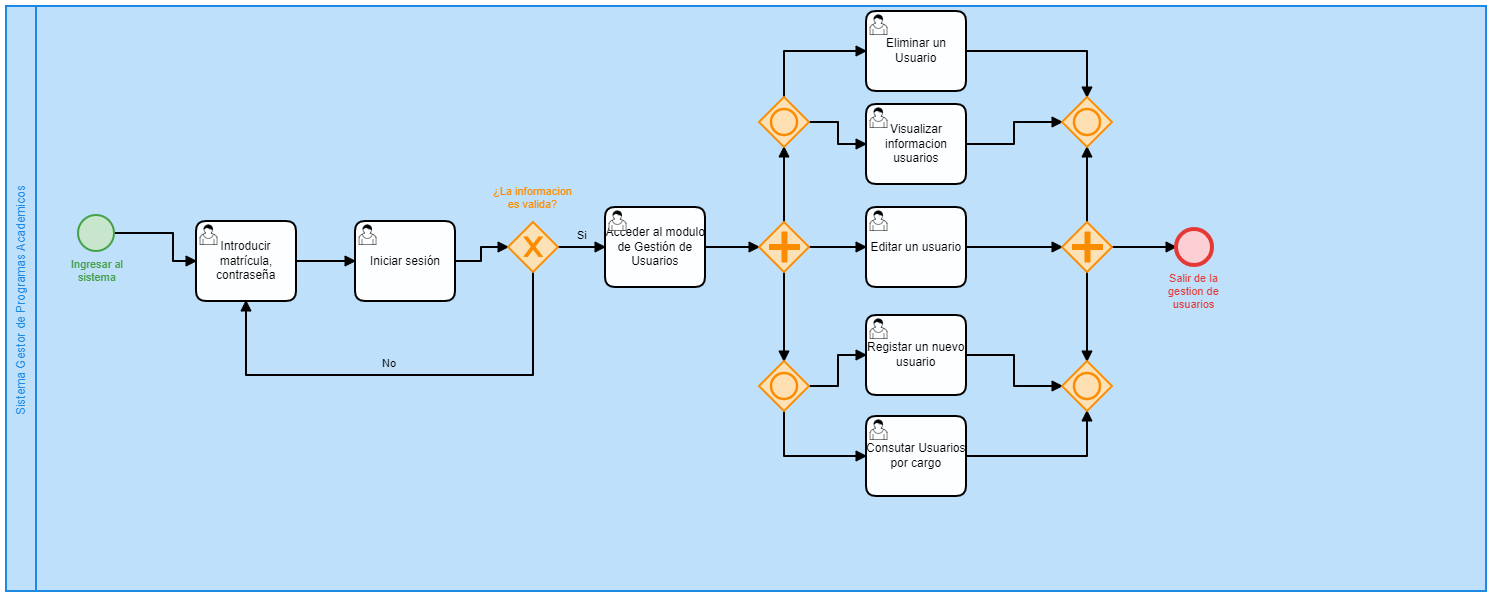
\includegraphics[width=\linewidth]{images/SP5/Gestion-Usuarios-proceso.png}}
        	\caption{Subproceso de la gestión de usuarios}
        	\label{BPMNGRH}
        \end{figure}
        
        El Jefe de Innovación Educativa de la Unidad Académica accede al Sistema Gestor de Programas Académicos.\\
        
        Ingresa su matrícula y contraseña para iniciar sesión. En caso de errores de validación de sus datos, debe intentarlo de nuevo.\\
        
        Ya dentro del sistema, accede a la sección llamada ''Gestión de Usuarios'' Aquí podrá consultar, visualizar, eliminar, modificar y agregar usuarios de la Unidad Académica bajo su cargo. \\
        
        Para agregar y/o editar un usuario, es necesario acceder a dos pantallas distintas. Es decir, no puede realizar ambas acciones de manera simultánea.\\
        
        En cambio, para consultar, visualizar y eliminar un usuario, sí es posible realizarlo en la misma pantalla.\\
        
        [Más adelante se explica con más detalle éstas operaciones dentro de las pantallas del sistema.]\\
        
		
        \subsubsection{Gestión de Programas Académicos}
        
        \begin{figure}[!hbtp]
        	\centering
        	\hypertarget{BPMNGPA}{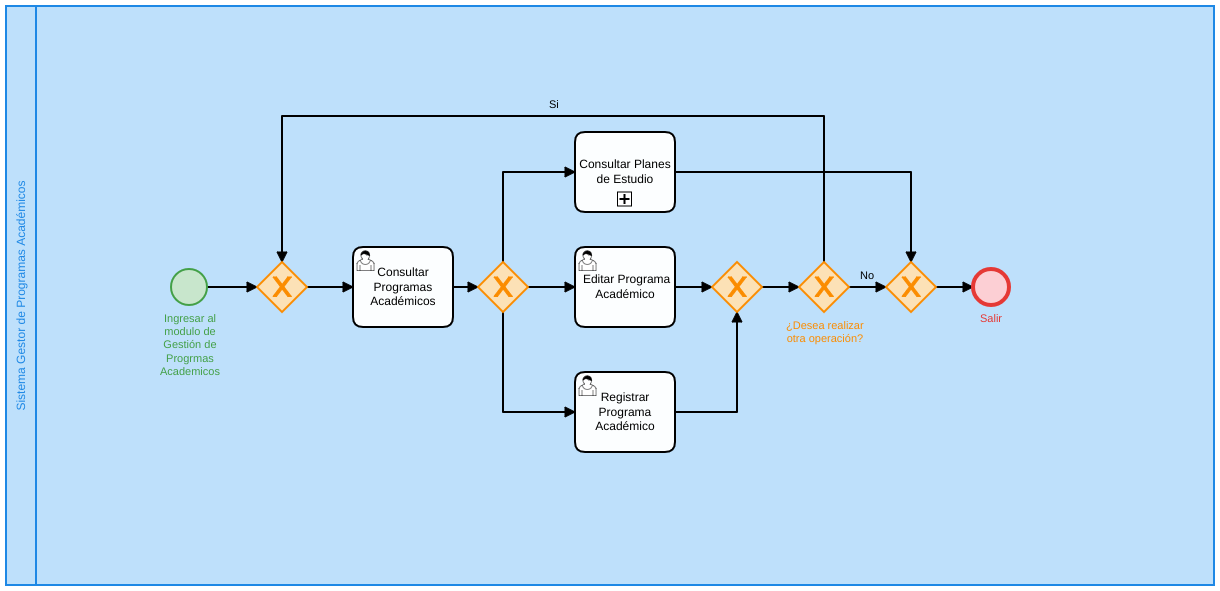
\includegraphics[width=\linewidth]{images/SP3/gestionPA.png}}
        	\caption{Subproceso de la gestión de Programas Académicos}
        	\label{BPMNGPA}
        \end{figure}
        
        El Jefe de Innovación Educativa de la Unidad Académica accede al Sistema Gestor de Programas Académicos.\\
        
        Ingresa su matrícula y contraseña para iniciar sesión. En caso de errores de validación de sus datos, debe intentarlo de nuevo.\\
        
        Ya dentro del sistema, accede a la sección llamada ''Gestión de Programas Académicos'' Aquí podrá consultar, visualizar, modificar y agregar Programas Académicos. \\
        
        Para agregar y/o editar un Programa Académico, es necesario acceder a dos pantallas distintas. Es decir, no puede realizar ambas acciones de manera simultánea.\\
        
        En cambio, para consultar y visualizar  un Programa Académico, sí es posible realizarlo en la misma pantalla.\\
        
        [Más adelante se explica con más detalle éstas operaciones dentro de las pantallas del sistema.]\\
        
        

